\documentclass[14pt]{matmex-diploma-custom}

\begin{document}

\filltitle{ru}{
    chair              = {Кафедра информатики},
    title              = {Разработка системы автоматического анализа новостных публикаций на финансовом рынке},
    %   coursework - Курсовая работа
    %   diploma - Диплом специалиста
    %   master - Диплом магистра
    %   bachelor - Диплом бакалавра
    type               = {bachelor},
    position           = {студента},
    group              = 13.Б09-мм,
    author             = {Зернов Алексей Викторович},
    supervisorPosition = {к.\,ф.-м.\,н., доцент},
    supervisor         = {Григорьев Д.\,А.},
    reviewerPosition   = {д.\,т.\,н., декан},
    reviewer           = {Мусаев А.\,А.},
%   chairHeadPosition  = {д.\,ф.-м.\,н., профессор},
%   chairHead          = {Новиков Б.\,А.},
    university         = {Санкт-Петербургский Государственный Университет},
    faculty            = {Математико-механический факультет},
    city               = {Санкт-Петербург},
    year               = {2017}
}
\filltitle{en}{
    chair              = {Computer Science Department},
    title              = {Development of the automatic analysis system of a financial market's news publications},
    type               = {bachelor},
    position           = {student},
    group              = {13.Б09-мм},
    author             = {Zernov Alexey Viktorovich},
    supervisorPosition = {Sc.\,C., associate professor},
    supervisor         = {Grigoryev D.\,A.},
    reviewerPosition   = {Sc.\,D., dean},
    reviewer           = {Musaev A.\,A.},
%   chairHeadPosition  = {professor},
%   chairHead          = {Boris Novikov},
    faculty            = {Faculty of Mathematics and Mechanics},
    city               = {Saint-Petersburg},
    year               = {2017}
}

\maketitle

\tableofcontents

\clearpage\section*{Введение}

\clearpage\section{Финансовый рынок}

В данном разделе будет представлен краткий обзор основных терминов, связанных с самим финансовым рынком, его структурой и основными участниками. Более подробная информация может быть получена в \cite{book:financial_market}.

\subsection{Определение}

В более общем виде \textbf{финансовый рынок}~--- совокупность экономических связей его участников, касающихся создания, поддержания и обращения капитала. Финансовый рынок является довольно абстрактным термином, и под ним часто подразумеваются более конкретные: рынок купонных и бескупонных облигаций, рынок акций (или фондовый рынок) или валютный рынок. Не смотря на выделение составляющих, каждая из них является частью единого механизма, в котором финансы перемещаются между каждым из конкретных рынков.

Каждый из финансовых рынков является рынком посредников между начальными владельцами финансов и их конечными пользователями. Если рынок основывается на финансах как на капитале, он называется фондовым рынком, и именно в этой роли выступает как составная часть всего финансового рынка.

В России финансовые рынки имеют следующие критерии, влияющие на их деятельность:

\begin{itemize}
\item Инвестиции в экономику страны
\item Международные рынки, влиние тенденций глобализации
\item Современные компьютерные технологии
\item Уровень комьютерной и информационной развитости участников рынков
\end{itemize}

\subsection{Структура}

Финансовый рынок может быть:

\begin{itemize}
\item Первичным или вторичным
\item Организованным или неорганизованным
\item Биржевым или внебиржевым
\item Традиционным или компьютеризированным
\item Кассовым или срочным
\end{itemize}

\textbf{Первичный рынок} обеспечивает выход ценных бумаг в оборот, это своеобразное <<производство>> ценных бумаг. На \textbf{вторичном рынке} в обороте находятся уже выпущенные ранее ценные бумаги. Вторичный рынок представляет из себя совокупность всех операций с данными ценными бумагами, в результате которых они переходят от одних владельцев к другим.

\textbf{Организованный рынок} отличается от \textbf{неорганизованного рынка} тем, что в первом имеются единые для всех участников рынка правила, за соблюдением которых следят организаторы. Во неорганизованном рынке соблюдение единых правил для всех участников рынка не гарантируется.

\textbf{Биржевой рынок}~--- такой рынок, на котором в качестве инструмента торговли используется аукцион. Руководителем же является некоторый специалист, например, NYSE\footnote{New York Stock Exchange~--- Нью-Йоркская фондовая биржа} или AMEX\footnote{American Stock Exchange - Американская фондовая биржа}. На \textbf{внебиржевых рынках} торги организуются при помощи электронных систем.

\textbf{Срочный рынок} чаще всего подразумевает отложенное исполнение сделки, в отличие от \textbf{кассового рынка}, когда сделки исполняются сразу. Обычно традиционные ценные бумаги (акции, облигации) идут в оборот на кассовом рынках, а контракты на производные инструменты рынка ценных бумаг~--- на срочных.

\subsection{Участники}

\textbf{Участники} рынка ценных бумаг~--- это физические лица или компании, которые продают или приобретают ценные бумаги, обеспечивают их оборот или расчеты по ним. 

Основными участниками рынка выступают \textbf{эмитенты}, выпускающие акции или облигации, с помощью которых привлекают финансирование, а также размещающие свободные на данный момент денежные средства. Эмитентами могут быть государство, субъекты государства или коммерческие предприятия. Целью эмитентов на первичном рынке является размещение запланированного транша по максимальной цене.

\textbf{Инвестор}~--- лицо, заинтересованное во вложении капитала в ценные бумаги. Их целью является как можно более выгодная покупка ценных бумаг максимально перспективных компаний.

\clearpage\section{Интеллектуальный анализ текста}

В настоящее время можно заметить увеличение роли компьютеров в жизни каждого человека. Инорфмация хранится преимущественно в цифровом виде, что значительно упрощает поиск или работу с ней. Но не смотря на это, многие данные все равно остаются довольно трудными для анализа, не смотря на оцифрованный вид, из-за чего можно подразделить из на следующие формы:

\begin{itemize}
\item Структурированные данные
\item Частично структурированные данные
\item Неструктурированные данные
\end{itemize}

Хорошим примером \textbf{структурированных данных} могут являться базы данных. \textbf{Частично структурированные данные}~--- это электронные письма, разнообразные файлы на языках разметок (HTML, XML и другие).

Если работа со структурированными или частично структурированными данными достаточно детерминированная, то \textbf{неструктурированные данные} представляют наибольший интерес в этом вопросе. Около 80\% корпоративных данных находится именно в неструктурированном формате, в котором сложно проводить поиск или извлекать необходимую информацию. Для этого нужны специфические методы и алгоритмы обработки. И поскольку самая популярная форма хранения информации~--- это текст, интеллектуальный анализ текста (text mining) является более важным процессом, нежели интеллектуальный анализ данных (data mining).

Интеллектуальный анализ текста стоит на пересечении дисциплин, включая в себя: обработку web-данных, информационный поиск, компьютерную лингвистику и обработку естественного языка.

\subsection{Процесс интеллектуального анализа текста}

Концепция интеллектуального анализа текста представлена в \cite{article:text_mining}. В интеллектуальном анализе текста можно выделить два основных этапа (Рис.~\ref{img:text_mining}):

\begin{itemize}
\item Фильтрация текста
\item Извлечение знаний
\end{itemize}

\begin{figure}[h]
\centering
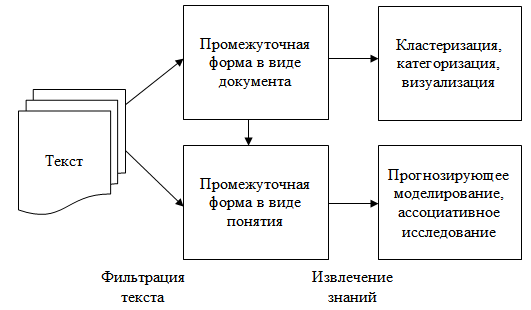
\includegraphics[width=0.7\textwidth]{img/text_mining}
\caption{Общий процесс интеллектуального анализа текста}
\label{img:text_mining}
\end{figure}

\textbf{Фильтрация} (или очистка) преобразует исходный текстовый документ в некоторое промежуточное представление. \textbf{Извлечение знаний}, в свою очередь, получает знания или некоторые шаблоны из уже промежуточного представления. Промежуточное представление может быть как структурированным, так и частично структурированным. Промежуточное представление может быть как новым текстовым документом, так понятием, в котором составляющие являются данными или наборами данных из какой-либо предметной области.

Анализ промежуточного представления документов выдает образцы и связи между всеми документами. Примеры задач: \emph{кластеризация}, \emph{визуализация} и \emph{категоризация документов}.

Анализ промежуточного представления понятий выдает образцы и связи между объектами или другими понятиями. Примеры задач: \emph{прогнозирующее моделирование} и \emph{ассоциативное исследование}.

Промежуточное представление в виде документа может быть преобразовано в промежуточное представление в виде понятия путем выделения релевантной информации, которая отношесится к необходимым объектам из какой-либо предметной области. Отсюда вытекает то, что промежуточное представление чаще не зависит от конкретное предметной области. К примеру, новостные потоки при фильтрации текста преобразуются в промежуточные представления в виде документов, соответствующим определенным статьям. Затем, в зависимости от поставленных задач визуализации или навигации, каждый документ (статья) проходит обработку знаний. Для извлечения же знаний в опрделеннной предметной области промежуточное представление в виде документа может быть преобразовано в промежуточное представление в виде понятия в соответствии с необходимыми требованиями. К примеру, можно извлечь информацию, касающуюся определенного товара или услуги из промежуточного представления в виде документа и сформировать базу данных товаров или услуг для предоставления знаний о них.

Ниже будут рассмотрены шаги, выполняемые при интеллектуальном анализе текста.

\subsubsection{Предварительная обработка текста}

Предварительная обработка включает в себя:

\begin{enumerate}
\item Токенизацию
\item Удаление <<стоп-слов>>
\item Определение происхождения слов
\end{enumerate}

\textbf{Токенизация}. Сначала текст разделяется на отдельные слова, освобождаясь от пробелов и знаков препинания.

\textbf{Удаление <<стоп-слов>>}. На этом этапе происходит избавление от <<ненужных>> конструкций текста. Это могут быть HTML или XML теги, предлоги, артикли и прочее.

\textbf{Определение происхождения слов} представляет из себя выявление корней определенных слов. Преимущественно встречаются два типа происхождения: флективный и деривационный.

\subsubsection{Преобразование текста}

Текстовый документ состоит из слов и информации об их происхождении. Два основных подхода представления документа: <<мешок слов>> (<<bag-of-words>>) и векторные пространства слов.

\subsubsection{Поиск признаков}

Под признаками можно понимать переменные. То есть в результате этого шага отбирается подмножество наиболее значимых признаков для их дальнейшего применения при построении моделей. Убираются, например, признаки, которые избыточны или не несут никакой информации.

\subsubsection{Методы анализа текста}

На данном шаге начинается построение модели с использованием разных методов, таких как кластеризация, классификация, информационный поиск и других. Данные методы распознавания данных также подходят и для интеллектуального анализа текста.

\subsubsection{Интерпретация и оценка}

На последнем шаге (в зависимости от того, что требуется) проводится анализ результатов.

\subsection{Области применения интеллектуального анализа текста}

Как уже упоминалось выше, интеллектуальный анализ текста стоит на пересечении разных дисциплин, включая в себя: извлечение информации, информационный поиск, обработку естественного языка и интеллектуальный анализ данных. Ниже будет подробнее рассказано о каждой из областей.

\subsubsection{Извлечение информации}

В процессе извлечения информации автоматически извлекается структурированная информация из неструктурированных данных. С помощью распознавания образов данная система определяет, например, где имена людей, где названия компаний, а где местоположение. То есть в документах происходит поиск предопределенных последовательностей. Подобное решение позволяет получить элементы, подходящие для использования в базах данных для дальнейшего хранения, анализа или обработки.

\subsubsection{Информационный поиск}

Наиболее известными системами информационного поиска являются поисковые системы Google. В данной задаче используются методы, используемые для хранения, представления и доступа к информации, которая преимущественно представлена в виде текстовых документов (а также новостных лент или книг), которые могут быть получены по запросу пользователя. Это своего рода расширение поиска по документам, позволяющее сужать набор документов, имеющих отношение к запросу пользователя. Эти системы значительно сокращают время, необходимое для поиска необходимой информации.

\subsubsection{Обработка естественного языка}

Данная задача представляет из себя самую активную проблему в области искусственного интеллекта. Цель: исследовать естественный язык так, чтобы у компьютеров была возможность понимать языки, подобные тем, что используют для общения люди. Обработка естественного языка включает в себя распознавание и генерацию, которые отвечают за такие способности компьютера как <<читать>> и <<говорить>> на естественном языке соответственно. Подобные системы включают в себя проверку грамматики, лексические, синтаксические и семантические анализаторы.

\subsubsection{Интеллектуальный анализ данных}

Данные задачи относятся к поиску знаний или релевантной информации в большом объеме данных. Система пытается обраружить правила (статистически) и образцы (автоматически) от данных. Подобные системы имеют возможность предсказания, основываясь на <<опыте>>, полученном в результате исследования.

\clearpage\section{Обзор существующих инструментов}

В данном разделе будут рассмотрены основные инструменты, представленные в виде библиотек или отдельных сервисов. Внимание уделено в основном инструментам, работающим с русским языком.

\subsection{Natural Language Toolkit}

NTLK\footnote{\url{http://www.nltk.org}} является пакетом библиотек и программ для разработки программ на Python, работающих с естественным языком. Сопровождается обширной документацией, а также книгой\footnote{\url{http://www.nltk.org/book/}}, объясняющей основные концепции проблем, для решения которых предназначен данный пакет. NTLK~--- свободное программное обеспечение, то есть доступное бесплатно.

Данный пакет подходит для таких областей как компьютерная лингвистика, эмпирическая лингвистика, когнитивистика, искусственный интеллект, информационный поиск и машинное обучение. NTLK используется преимущественно в качестве учебного пособия, индивидуального обучения или прототипирования и создания систем, ориентированных на научно-исследовательскую деятельность.

Изначально пакет предназначен для англоязычных текстов, но имеется возможность обучения классификаторов для остальных языков.

\subsection{pymorphy2}

Pymorphy2\footnote{\url{https://pymorphy2.readthedocs.io/en/latest/index.html}}\cite{tools:pymorphy2} написан на языке Python и имеет следующие возможности:

\begin{itemize}

\item Приведение слова к нормальной форме

\item Ставить слово в нужную форму

\item Возвращать грамматическую информацию о слове

\end{itemize}

Распространяется pymorphy2 под лицензией MIT\footnote{\url{https://opensource.org/licenses/MIT}}, если используется в научной работе.

\subsection{Томита-парсер}

Томита-парсер\footnote{\url{https://tech.yandex.ru/tomita/}} способен извлекать структурированные данные из текстов на естественном языке. Как и почти во всех инструментах, рассматриваемых в данном разделе, Томита-парсер ориентирован преимущественно на русскоязычные тексты. В нем используются контекстно-свободные грамматики и словари ключевых слов. Код проекта\footnote{\url{https://github.com/yandex/tomita-parser/}} находится в свободном доступе.

\subsection{Яндекс.Спеллер}

Яндекс.Спеллер\footnote{\url{https://tech.yandex.ru/speller/}} выполняет задачу проверки орфографии в текстах на английском, русском и украинском языках. Для этого используется орфографический словарь. К тому же, предоставлен набор API методов для реализации данной проверки разработчиками сайтов или приложений.

\subsection{OntosMiner}

OntosMiner\footnote{\url{http://my-eventos.com/solution/ontosminer/}} является решением компании Eventos\footnote{\url{http://my-eventos.com/solution/ontosminer/}}, занимающейся в большей степени разработкой продуктов в области лингвистического анализа текстовой информации, кластеризацией и классификацией информации. Конкретно OntosMiner является целой комплексной системой, дающей возможность распозавания связей между сущностями в текстах на естественной языке. Также, она позволяет определеять общую тональность текста.

\clearpage\section{Теоретическая информация}

\clearpage\section{Практическая часть}

\clearpage\section*{Заключение}

\setmonofont[Mapping=tex-text]{CMU Typewriter Text}
\bibliographystyle{ugost2008ls}
\bibliography{diploma}

\end{document}
